\documentclass{beamer}

\usetheme[]{Copenhagen}
\usepackage[utf8]{inputenc}
\usepackage{graphicx}
\usepackage{tikz}
\title[]{GNU/LINUX}
\subtitle{qué es, de dónde viene y cómo se instala} % Opcional
\author{Sergio Carlón Ruiz}
\institute{Grupo universitario de Informática} % Opcional

\begin{document}

\begin{frame}
\titlepage
\end{frame}

%------------------------------------------------------------------
\begin{frame}{El primer culpable: Richard Stallman}
  \begin{columns}[T]
    \begin{column}{.5\textwidth}
     En 1971, según estudiaba su primer año de física, Stallman 
     se convierte en "hacker" 
     del Laboratorio de inteligencia artificial del MIT.
 	
 	Entre 1982 y 1983, luchó contra el monopolio de Symbolics, una empresa constituida por antiguos compañeros suyos, que pretendía privatizar todo el software que se utilizaba en los laboratorios del MIT.

    \end{column}
    \begin{column}{.5\textwidth}
    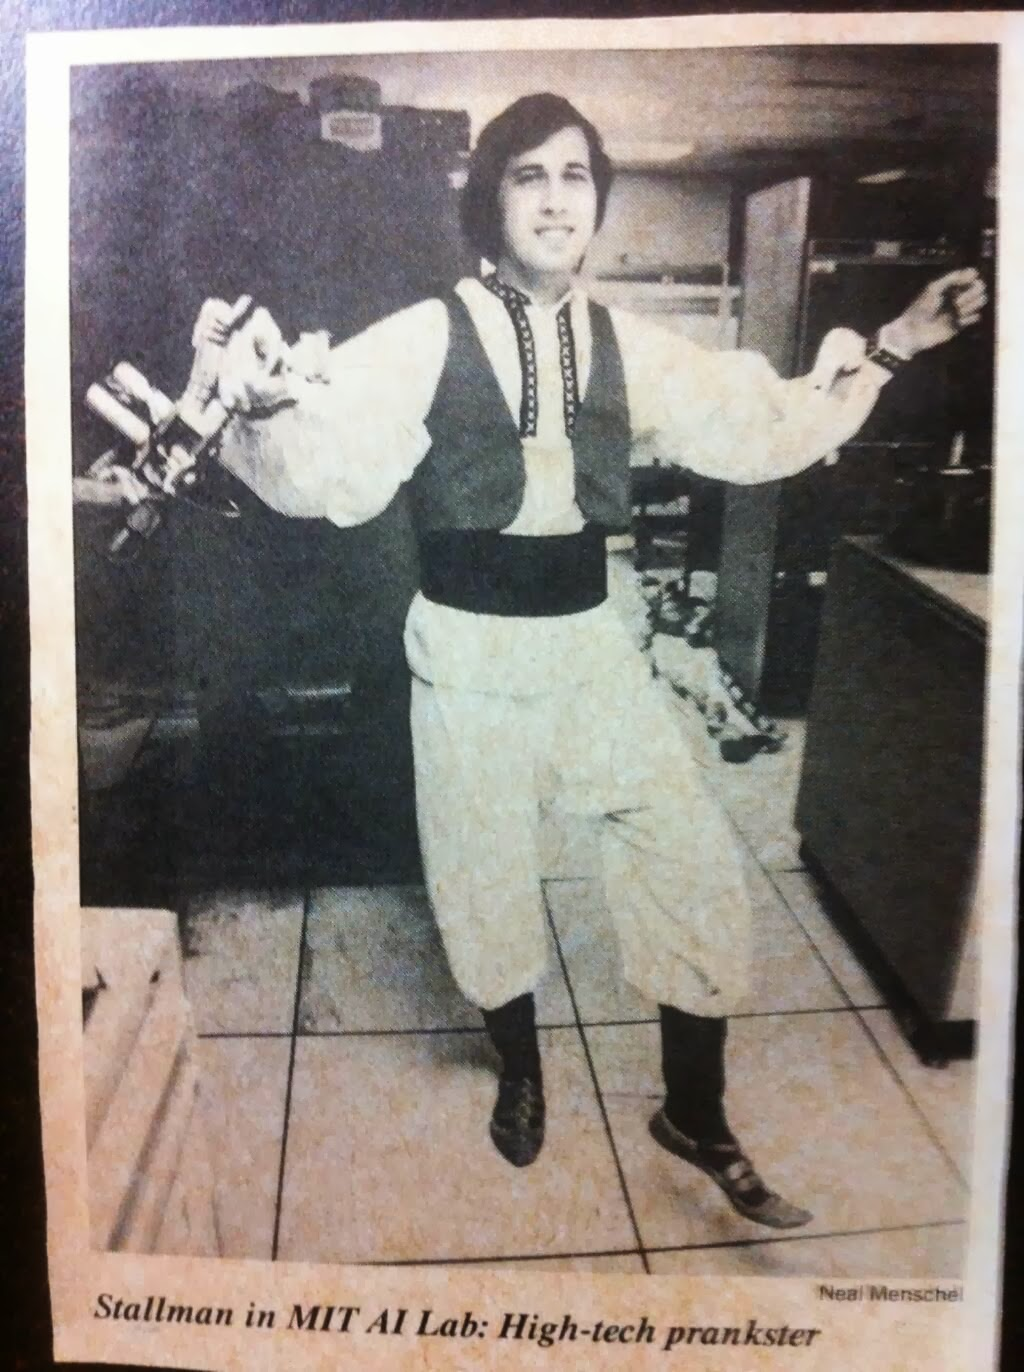
\includegraphics[width=\textwidth]{stallman_joven.jpg}
    \end{column}
  \end{columns}
\end{frame}
%-----------------------------------------------------------------
\begin{frame}
\frametitle{\centerline{Software Libre}}
 \begin{columns}[T]
  \begin{column}{.5\textwidth}
   \begin{itemize}
    \item \textbf {Libertad 0}: la libertad para ejecutar el programa sea cual sea nuestro propósito.
    \item \textbf {Libertad 1}: la libertad de estudiar cómo funciona el programa y modificarlo, adaptándolo a las propias necesidades
    \item \textbf{Libertad 2}: la libertad para redistribuir copias y ayudar así a tu vecino.
    \item \textbf {Libertad 3}:la libertad para mejorar el programa y luego publicarlo para el bien de toda la comunidad
   \end{itemize}  	
  \end{column}
  \begin{column}{.5\textwidth}
   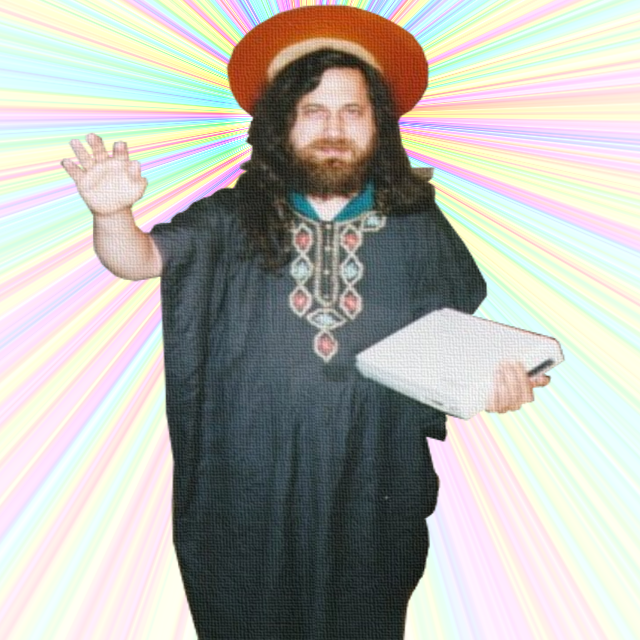
\includegraphics[width=\textwidth]{sanignucio.png}
  \end{column} 
 \end{columns}
\end{frame}
%------------------------------------------------------------------

\begin{frame}{El Manifiesto GNU}{GNU Not UNIX}
\begin{center}

\includegraphics[scale=0.055]{gnu.png}
\end{center}
En 1983 anunció el proyecto GNU, y en 1984 dejó su trabajo en el MIT para dedicarse por completo a su ambicioso proyecto, un sistema operativo de
tipo UNIX que permitiera compartir a los hackers
\begin{itemize}
\item (Publicado en 1984) marca el inicio del movimiento GNU y sienta las bases de los objetivos de dicho movimiento; así como la respuesta a las preguntas frecuentes que surgirían
\item En 1985 funda la "Free Software Foundation" FSF
para dar soporte económico y legal  al proyecto GNU
\item Aparición de: GNU Emacs; GCC
\end{itemize}
\end{frame}

%------------------------------------------------------------------
\begin {frame}{Qué es UNIX}
Unix (registrado oficialmente como UNIX®) es un sistema operativo portable, multitarea y multiusuario; desarrollado, en principio, en 1969, por un grupo de empleados de los laboratorios Bell de AT\&T, entre los que figuran Ken Thompson, Dennis Ritchie y Douglas McIlroy
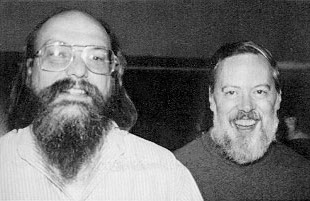
\includegraphics[scale=0.7]{ritchie.jpg}
\end{frame}

\begin{frame}{Existen muchos derivados de UNIX}
 \begin{itemize}
 \item \textbf{Minix}, creado por Tanenbaum con fines pedagógicos.
 
\includegraphics[scale=0.15]{minix.png}
 \item\textbf{BSD}, otra familia de la que provienen FreeBSD, OpenBSD y OSX
 
\includegraphics[scale=0.3]{beastie.png}
 \item\textbf{LINUX}, publicado en 1991 por Linus Torvalds 
\begin{tikzpicture}[remember picture,overlay]  
  \node [xshift=-2cm,yshift=2cm] at (current page.south east)
    {
\includegraphics[scale=0.2]{tux.png}};
\end{tikzpicture}
 \end{itemize}
\end{frame}
%------------------------------------------------------------------

\begin{frame}{Todo estaba listo}{¿todo?}
En 1990 estaban desarrollados casi todos los componentes para crear un sistema completo GNU

Pero faltaba una cosa: el núcleo (Kernel)

Hubo muchos intentos fallidos: Alix, GNU Hurd
\begin{tikzpicture}[remember picture,overlay]  
  \node [xshift=-2cm,yshift=3cm] at (current page.south east)
    {
\includegraphics[scale=0.05]{hurd.png}};
\end{tikzpicture}

\end{frame}

\begin{frame}{Linus Torvalds}
Estudiante de Ciencias de la Computación de la Universidad de Helsinki (Finlandia)
En 1991 sube la versión 0.01 de "Freax" en el ftp de su escuela

Creado como hobby para sustituir MINIX

En 1992 apareció la unión \textbf{GNU/Linux}

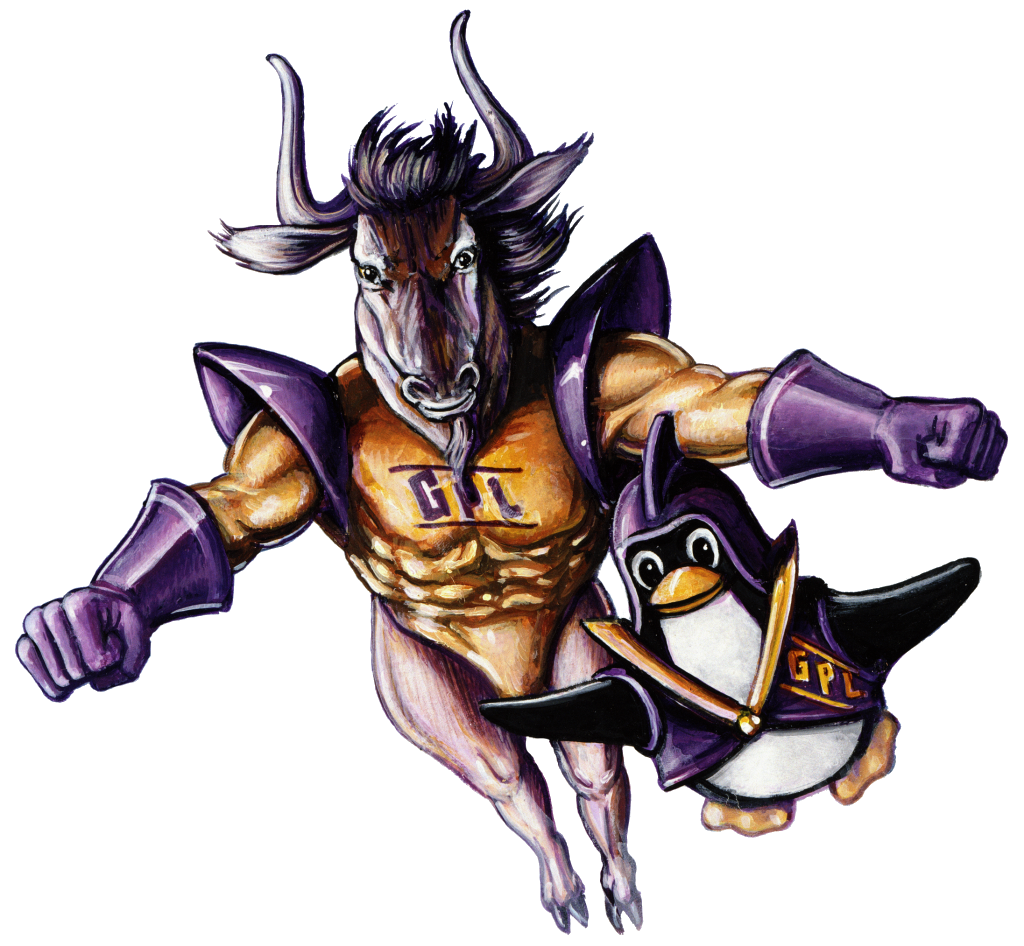
\includegraphics[scale=0.12]{tux_gnu.png}
\begin{tikzpicture}[remember picture,overlay]  
  \node [xshift=-3cm,yshift=-2cm] at (current page.east)
    {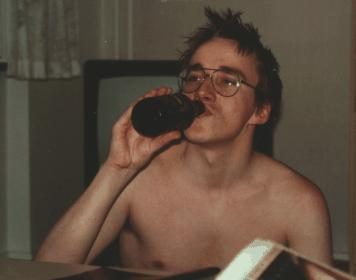
\includegraphics[scale=0.4]{linus_beer}};
\end{tikzpicture}
\end{frame}

\begin{frame}{Distribución GNU/Linux}
Una distribución GNU/Linux, es una distribución de software basada en el núcleo Linux que incluye determinados paquetes de software GNU para satisfacer las necesidades de un grupo específico de usuarios

\begin{columns}[t]
\column{.05\textwidth}
\centering

\includegraphics[scale=0.08]{debian.png}\\

\includegraphics[scale=0.08]{ubuntu.png}
\column{.05\textwidth}
\centering

\includegraphics[scale=0.09]{redhat.png}\\

\includegraphics[scale=0.09]{gentoo.png}
\column{.05\textwidth}
\centering

\includegraphics[scale=0.03]{slackware.png}\\

\includegraphics[scale=0.03]{arch.png}
\end{columns}

\end{frame}
%--------------------------------------------------
\begin{frame}{Vuestra situación...}

\includegraphics[width=\textwidth]{distroseverywhere.jpg}
\end {frame}

%--------------------------------
\begin{frame}{Miedos Absurdos}{instalar una distro}
\begin{itemize}
	\item Me borrara mi windows 
	\item Me estropeará el mac 
	\item no encontraré programas
	\item no podré pagar por software
\end{itemize}
\end{frame}

\begin{frame}{Pero lo cierto es que..}{}
\begin{itemize}
\item casi cualquier distro GNU/Linux respetará el sistema que tengas ya instalado (dual boot, ya sea EFI o MBR)
\item puedes probarlo sin instalarlo (vía live USB o CD/DVD)
\item encontrarás millones de programas muy útiles, y además dispondrás del código
\end{itemize}
\end{frame}
%---------------------------------------------------------------------
\begin{frame}{Relax...}
\begin{center}
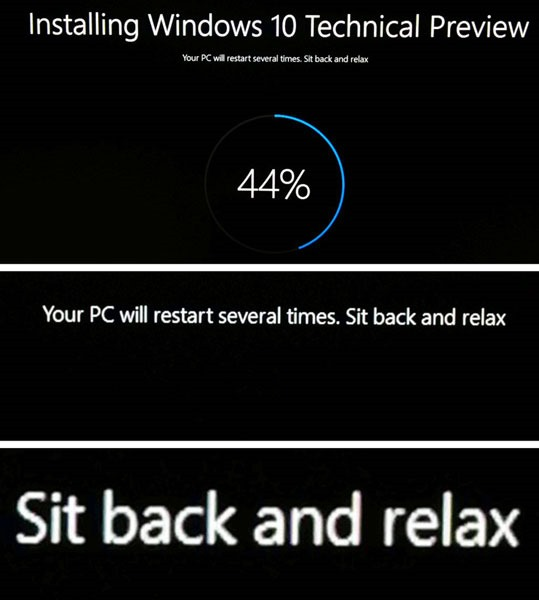
\includegraphics[height=7cm,keepaspectratio]{relax.jpg}
\end{center}
\end {frame}

\begin{frame}{NOW Im relaxed}
\begin{center}
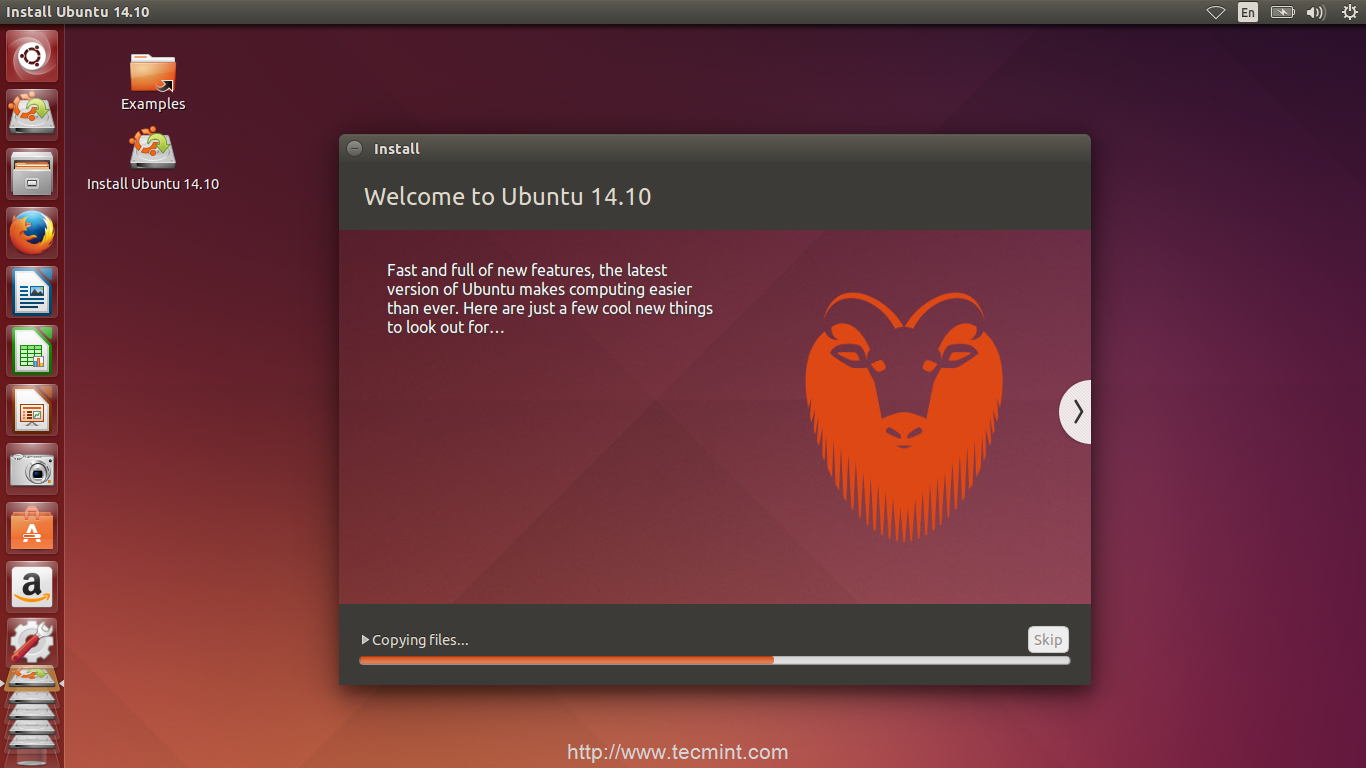
\includegraphics[width=\textwidth]{install.png}
\end{center}
\end {frame}

%---------------------------------------------------------------------

\begin{frame}{Keeping relaxed}{}
\begin{center}
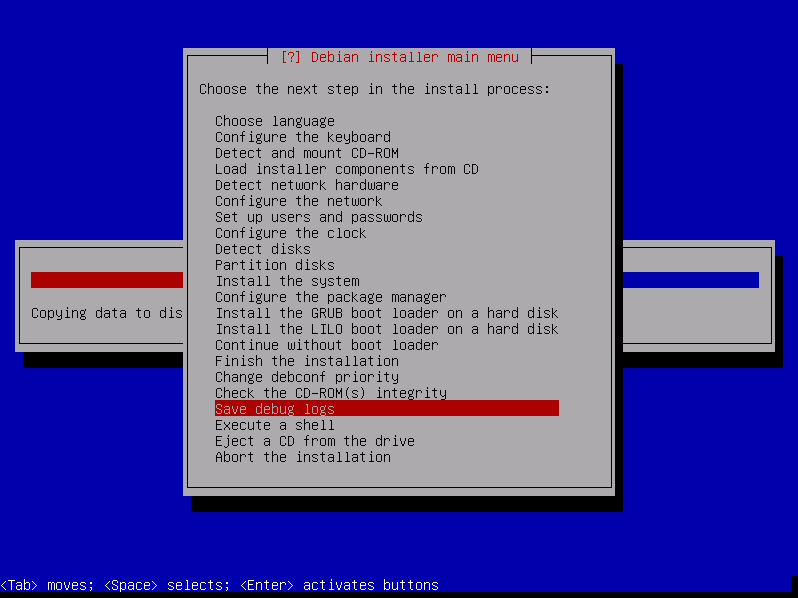
\includegraphics[height=7cm,keepaspectratio]{installconsole.png}
\end{center}
\end {frame}

\begin {frame}{Revolution OS}
\begin {itemize}
\item Kernel 4.9 (Next LTS)
\item Steam OS 
\item Polémica sobre winodws 10
\item Amdgpu, biblioteca Vulkan 
\item AWS (amazon web services)
\item Supercomputadora Sunway TaihuLight, Raise OS (Linux)

\end{itemize}
\end {frame}
%----------------------------------------------------------
\begin {frame}{Cosas serias...}{www.top500.org}
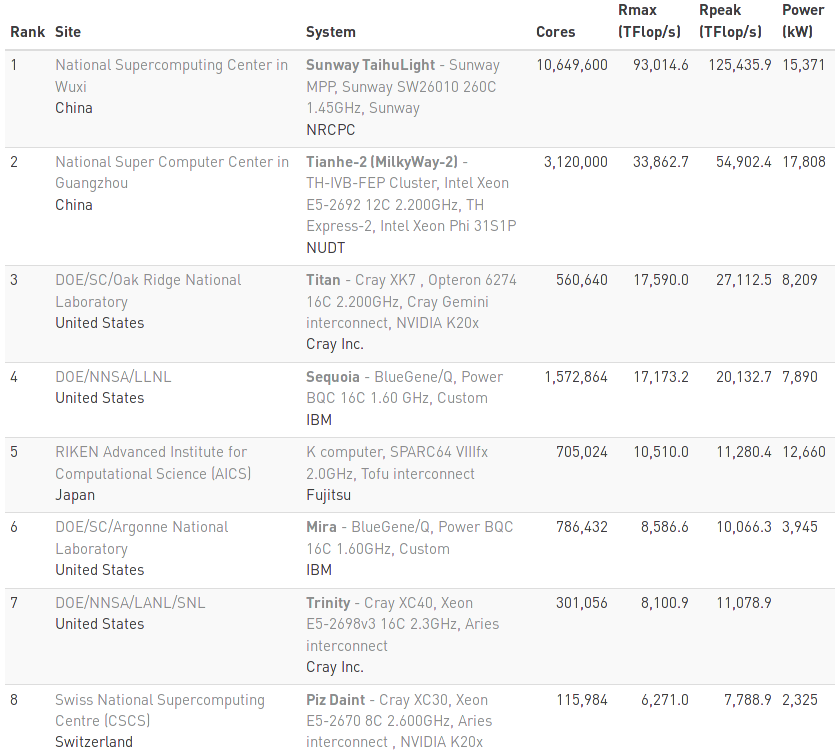
\includegraphics[width=\textwidth]{top.png}
\end {frame}

\begin{frame}{Revolution OS}{En serio..}

\includegraphics[width=\textwidth]{micro.png}
\end {frame}

%----------------------------------------------------------------------
\begin{frame}{¿Y como se instala?}{}
\begin{itemize}
\item Cogemos una torre un portátil, con unos cuantos GBs libres, es difícil determinar cuántos, depende de lo que instales.
\item Te haces con una .iso
\item Cargas las iso desde un CD/DVD, USB...
\item Sigues las instrucciones que aparecen.
\end{itemize}
\end{frame}
%----------------------------------------------------------------------

\begin{frame}{Nestro amigo el UEFI}
\begin{itemize}
\item Creado a mediados de los 90
\item Presente en los mac en los 90 y en los pc's con la salida de Windows 8
\item Propósito sustituir a la BIOS
\item El Secure Boot se encaga de que el sistema solo arranque cosas "seguras" 
\end{itemize}
\end{frame}

%----------------------------------------------------------
\begin {frame}
\frametitle{\centerline{Un dia Feliz}}
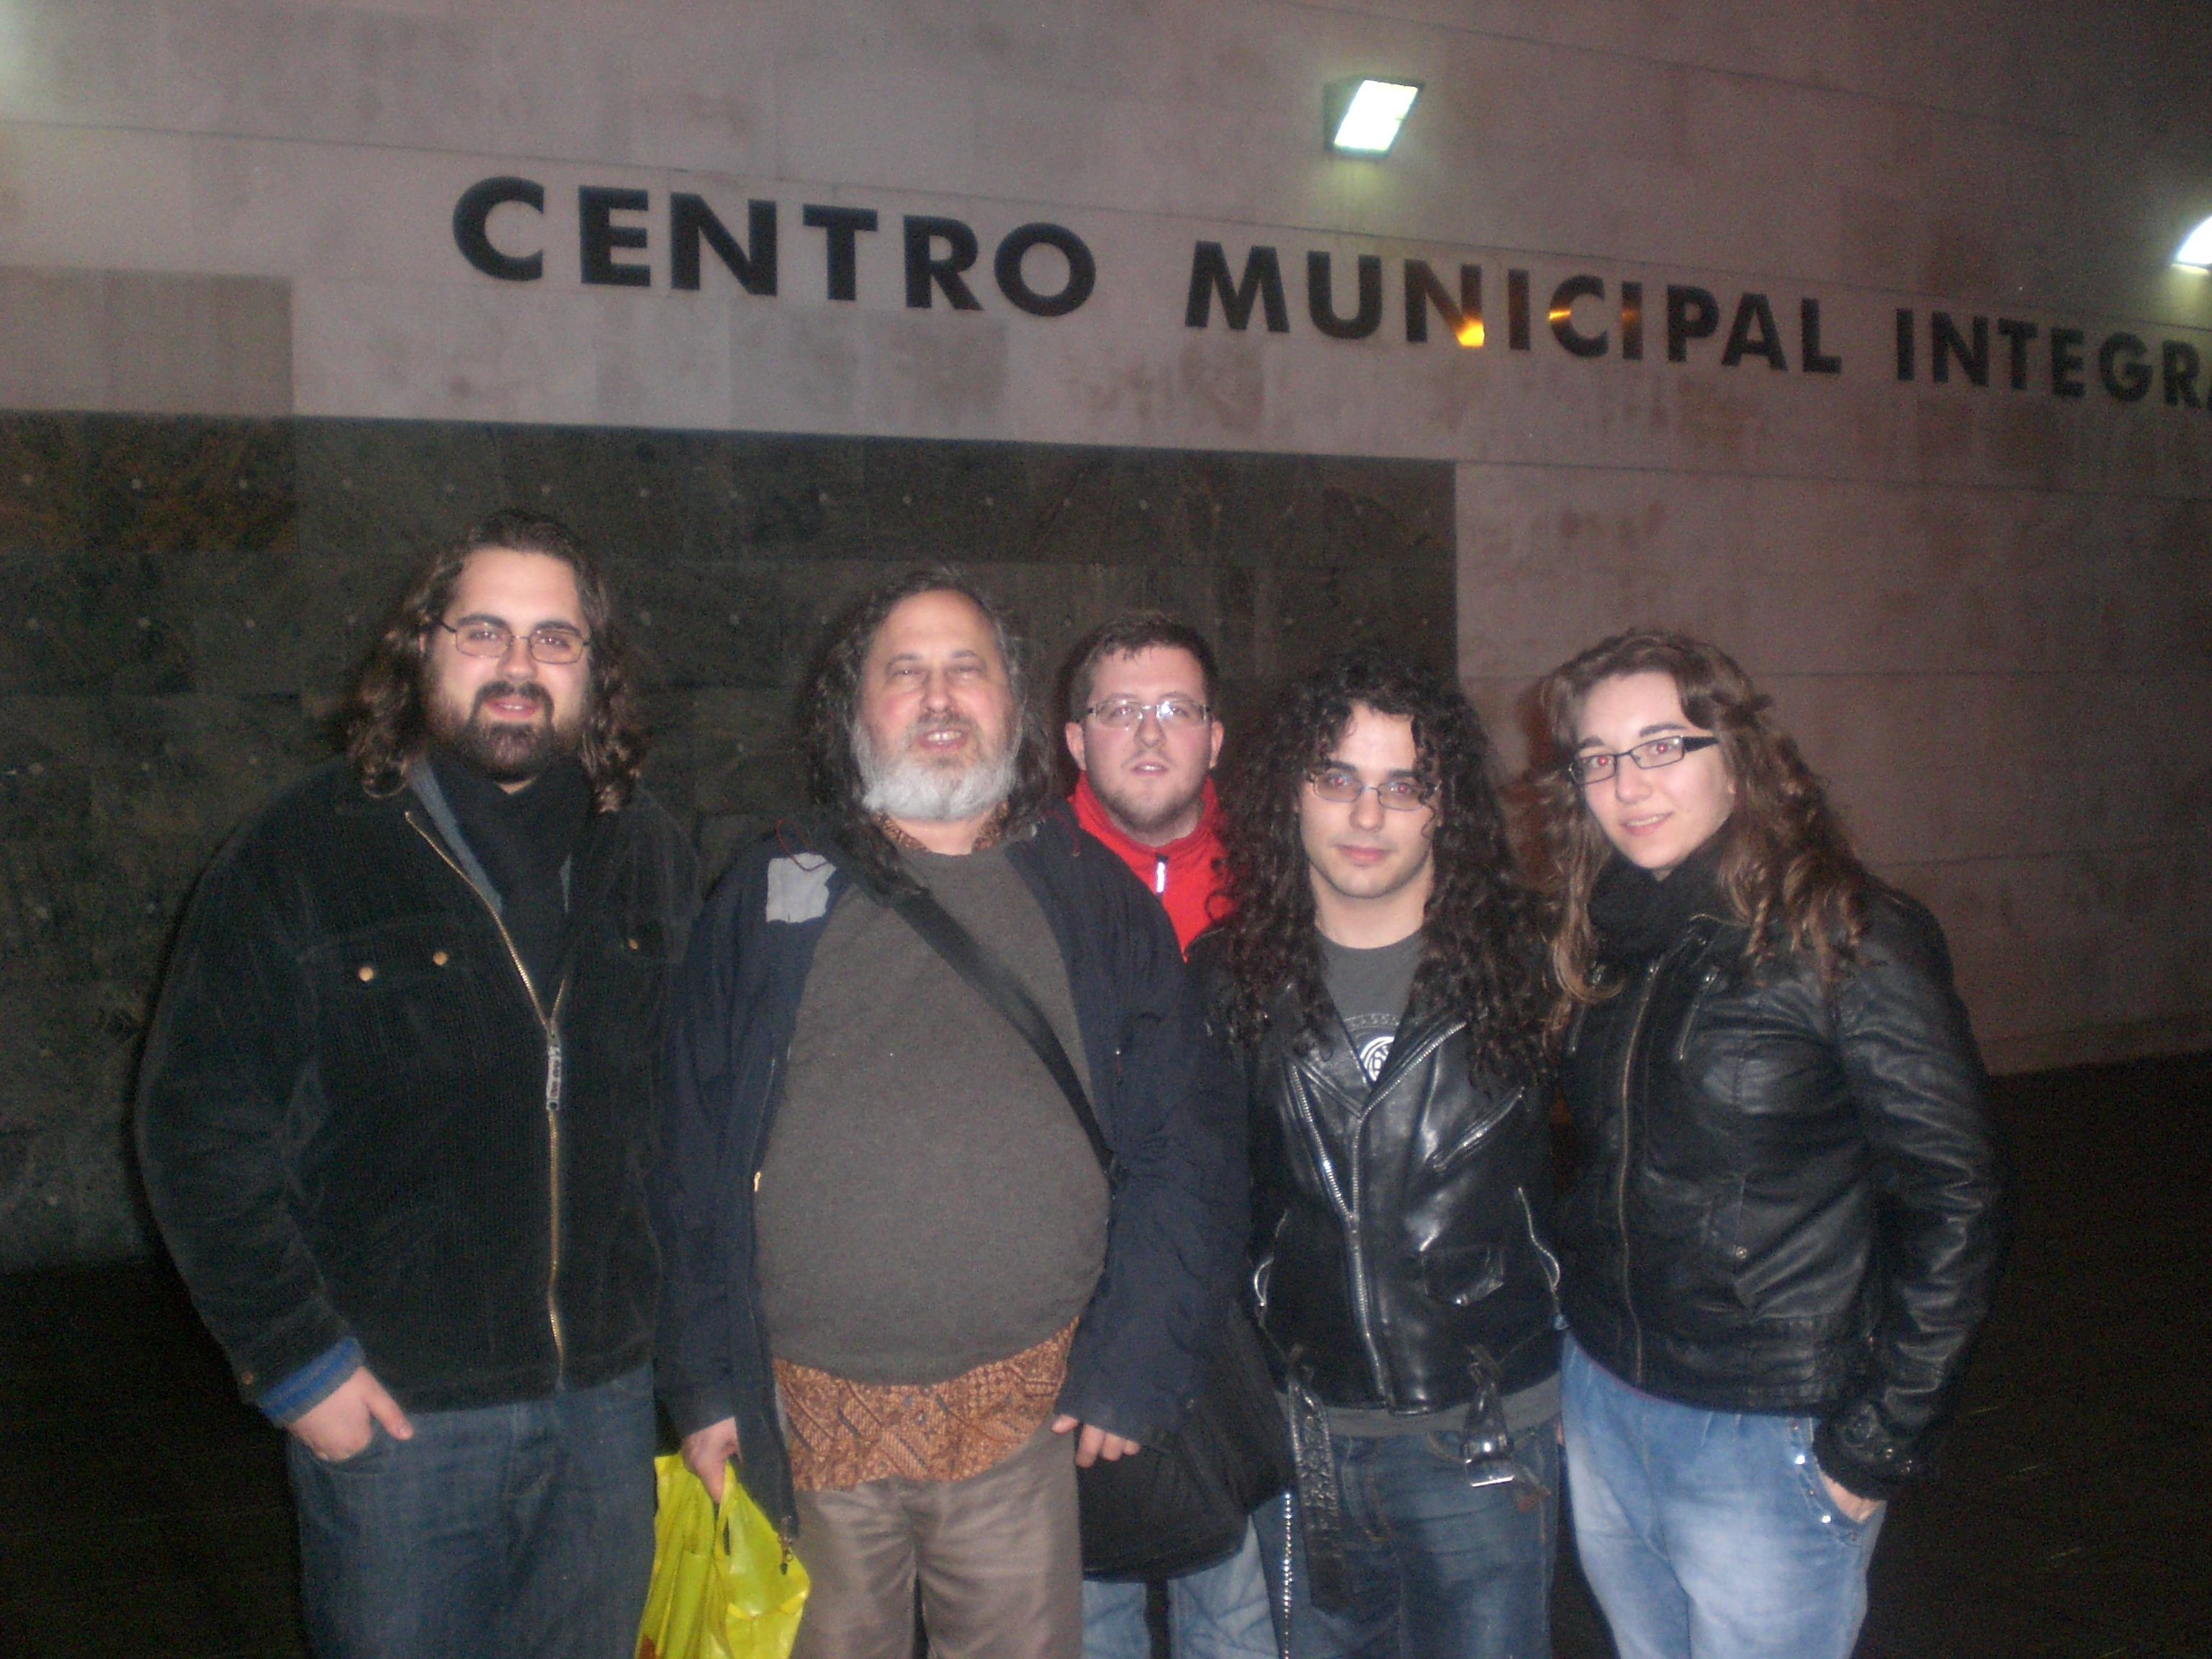
\includegraphics[width=\textwidth]{gijon.jpg}
\end {frame}
%------------------------------------------------
\begin {frame}
\frametitle{\centerline{}}
\begin{center}
\begin{center}\huge ¿Alguna pregunta? \end{center}
 \begin{figure}

\includegraphics[scale=0.90]{guino.png}
\end{figure}
\end{center}
\end {frame}
%----------------------------------------------------------
\begin{frame}
\begin{center}\huge ¡Gracias por asistir!\end{center}
\begin{center}
\includegraphics[scale=0.5]{gui.png}\end{center}
\begin{center}Ahora, a continuación, tenemos Install Party en la sala Hedy Lamarr :D\end{center}
\begin{center}\huge Happy Hacking!\end{center}

\end{frame}

%Trasparencias
\end{document}
